Das Verfahren zur Bestimmung der deflektometrischen Registrierung wurde in Kapitel \ref{chp:deflektometrischeRegistrierung} eingeführt und bestimmt eine Zuordnung zwischen Bildschirm- und Kamerapunkten.
Nach Abschnitt \ref{sec:auswertungDeflektometrischeRegistrierung} lässt sich diese Zuordnung durch zwei Bilder darstellen und mittels Methoden aus der Bildverarbeitung auswerten.
Die Parameter zur Erzeugung der Muster nach Gleichung \ref{eq:monitormuster_mehrstufig} können in Tabelle \ref{tab:paramSichtpruefung} abgelesen werden.

\begin{table}[H]
	\centering
	\begin{tabular}{lll}
	\hline 
	\textbf{Beschreibung} & \textbf{Name} & \textbf{Wert} \\ 
	\hline 
	Amplitude (beeinflusst die Helligkeit) & $A_m$ & 127.5 \\
	Kontrast & $C_m$ & 1.0 \\
	Anzahl Perioden des ersten Muster & $N_p^1$ & 3 \\ 
	Anzahl Perioden des zweiten Muster & $N_p^2$ & 5 \\ 
	Anzahl Perioden des dritten Muster & $N_p^3$ & 7 \\  
	Anzahl Phasenverschiebungen jedes Musters & $N_{shift}$ & 4 \\ 
	Bildschirmbreite (in Pixel) & \acrshort{lwidth} & 1920 \\
	Bildschirmhöhe (in Pixel) & \acrshort{lheight} & 1080 \\
	\hline 
	\end{tabular} 
	\caption{Parameter der Streifenmuster für das Verfahren \glqq Bestimmung der deflektometrischen Registrierung\grqq.}
	\label{tab:paramDeflektometrischRegistrierung}
\end{table}

\noindent
Durch diese Parameter erhält man eine Sequenz aus 12 Mustern, die auf einem LCD-Bildschirm angezeigt und anschließend durch eine Kamera aufgenommen werden können.
Zur Kodierung der Oberfläche werden insgesamt 256 Helligkeitsstufen auf die Oberfläche abgebildet.

\p
Im Folgenden wird nur die deflektometrische Registrierung der Zeilen untersucht.
Die Ergebnisse der deflektometrischen Registrierung der Spalten liefert für die Auswertung ähnliche Ergebnisse, weshalb darauf verzichtet wird.

% Durchlichtauswertung
{
	\FloatBarrier
    \subsection{Durchlichtauswertung}
    \label{sub:durchlichtAuswertungDeflektometrischeRegistrierung}
    Wie auch im Abschnitt \ref{sec:ergebnisseSichtpruefungDurchLichtstreuung} soll das Verfahren zunächst mit der Durchlichtauswertung für transparente Objekte durchgeführt werden.
Für einen nachfolgenden Vergleich sollen mit dem Verfahren auch das Brillenglas 1 und das Brillenglas 2 aus Abbildung \ref{tikz:abbStreifenaufnahmen} ausgewertet werden.
Zusätzlich zu den beiden Objekten wird ein anderes Brillenglas mit diesem Verfahren untersucht.
Es wird der Aufbau aus dem linken Teilbild aus Abbildung \ref{tikz:abbAufbauFotos} verwendet und die Brillengläser auf der Halterung positioniert.
Die Brillengläser werden zur Demonstration bei der Anzeige eines einzelnen Streifenmusters nach den Parametern aus Tabelle \ref{tab:paramDeflektometrischRegistrierung} aufgenommen:

% Abbildung: Aufnahmen mit sinusoidalen Streifenmustern
{
	\begin{figure}[H]
		\centering
		\begin{adjustbox}{width=\textwidth}
	\begin{tikzpicture}[every node/.style={inner sep=0,outer sep=0}]
		% Bilder
		\node [anchor=north west] (img1) at (0,0) {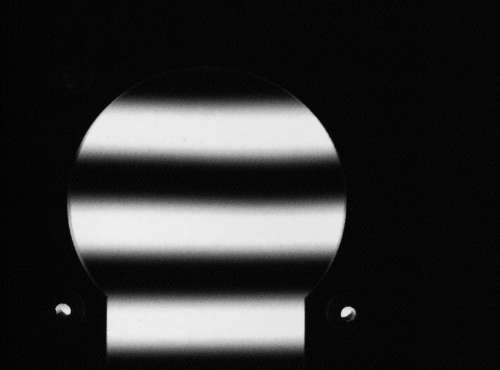
\includegraphics[width=.31\textwidth]{05_ergebnisse/ergDeflektometrischeRegistrierung/durchlichtAuswertungDeflektometrischeRegistrierung/figures/brillenglas_1_streifenmuster}};
		
		\node [anchor=north west] (img2) at (0.345\textwidth,0) {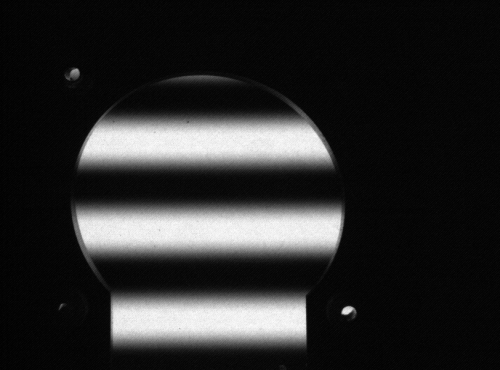
\includegraphics[width=.31\textwidth]{05_ergebnisse/ergDeflektometrischeRegistrierung/durchlichtAuswertungDeflektometrischeRegistrierung/figures/brillenglas_2_streifenmuster}};
		
		\node [anchor=north west] (img3) at (0.69\textwidth,0) {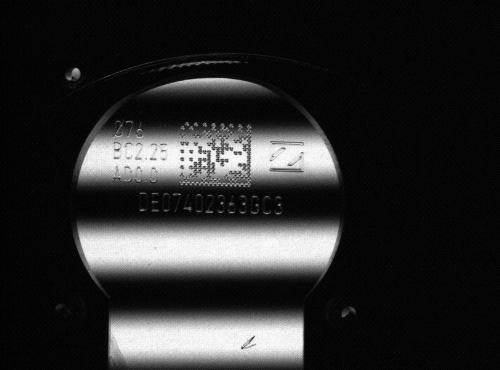
\includegraphics[width=.31\textwidth]{05_ergebnisse/ergDeflektometrischeRegistrierung/durchlichtAuswertungDeflektometrischeRegistrierung/figures/brillenglas_4_streifenmuster}};
		
		% Captions
		\node [below=0.2cm of img1] (cap1) {Brillenglas 1};
		\node [below=0.2cm of img2] (cap2) {Brillenglas 2};
		\node [below=0.2cm of img3] (cap3) {Brillenglas 4};			
	\end{tikzpicture}
\end{adjustbox}
\caption[Aufnahmen der Brillengläser bei der Durchlichtauswertung mit sinusoidalen Streifenmustern]{Aufnahmen der Brillengläser bei der Durchlichtauswertung mit sinusoidalen Streifenmustern}
		\label{tikz:abbSinusStreifenaufnahmen}
	\end{figure}
}

\noindent
Nach der Bestimmung der deflektometrischen Registrierung können daraus Bilder erstellt werden (siehe Definition \ref{def:graphDeflektometrischeRegistrierung}):

% Abbildung: Bilder der deflektometrische Registrierung der Zeilen
{
	\begin{figure}[H]
		\centering
		\begin{adjustbox}{width=\textwidth}
	\begin{tikzpicture}[every node/.style={inner sep=0,outer sep=0}]
		% Bilder
		\node [anchor=north west] (img1) at (0,0) {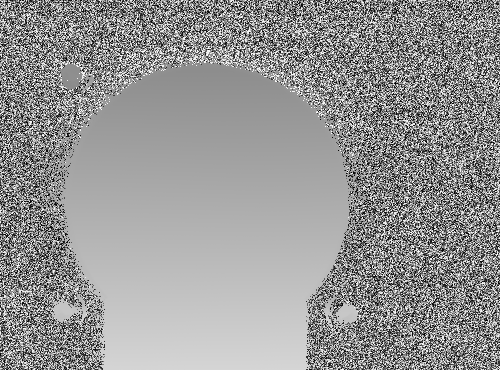
\includegraphics[width=.31\textwidth]{05_ergebnisse/ergDeflektometrischeRegistrierung/durchlichtAuswertungDeflektometrischeRegistrierung/figures/brillenglas_1_registrierung}};
		
		\node [anchor=north west] (img2) at (0.345\textwidth,0) {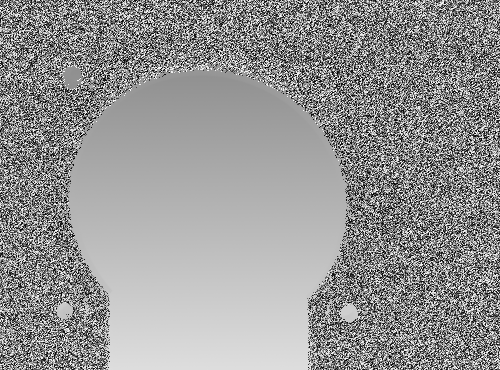
\includegraphics[width=.31\textwidth]{05_ergebnisse/ergDeflektometrischeRegistrierung/durchlichtAuswertungDeflektometrischeRegistrierung/figures/brillenglas_2_registrierung}};
		
		\node [anchor=north west] (img3) at (0.69\textwidth,0) {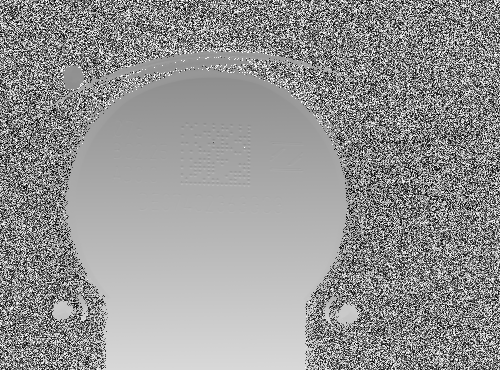
\includegraphics[width=.31\textwidth]{05_ergebnisse/ergDeflektometrischeRegistrierung/durchlichtAuswertungDeflektometrischeRegistrierung/figures/brillenglas_4_registrierung}};
		
		% Captions
		\node [below=0.2cm of img1] (cap1) {Brillenglas 1};
		\node [below=0.2cm of img2] (cap2) {Brillenglas 2};
		\node [below=0.2cm of img3] (cap3) {Brillenglas 4};			
	\end{tikzpicture}
\end{adjustbox}
\caption[Bilder der deflektometrischen Registrierung der Zeilen bei der Durchlichtauswertung]{Bilder der deflektometrischen Registrierung der Zeilen bei der Durchlichtauswertung.}
		\label{tikz:abbDeflectometricRegistrations}
	\end{figure}
}

\noindent
Zur Verdeutlichung der Ergebnisse des Verfahrens ist es sinnvoll die Ableitung der Bilder in Richtung der Zeilen zu bilden.
Mit Nachbearbeitung der Bilder der Ableitungen erhält man folgende Bilder:

% Abbildung: Bilder der deflektometrische Registrierung der Zeilen
{
	\begin{figure}[H]
		\centering
		\begin{adjustbox}{width=\textwidth}
	\begin{tikzpicture}[every node/.style={inner sep=0,outer sep=0}]
		% Bilder
		\node [anchor=north west] (img1) at (0,0) {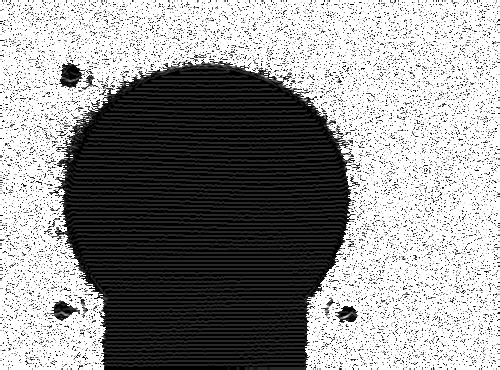
\includegraphics[width=.31\textwidth]{05_ergebnisse/ergDeflektometrischeRegistrierung/durchlichtAuswertungDeflektometrischeRegistrierung/figures/brillenglas_1_ableitung}};
		
		\node [anchor=north west] (img2) at (0.345\textwidth,0) {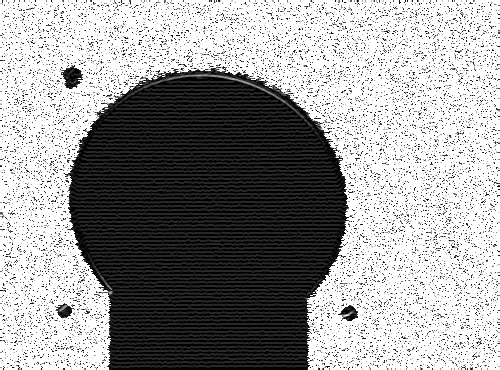
\includegraphics[width=.31\textwidth]{05_ergebnisse/ergDeflektometrischeRegistrierung/durchlichtAuswertungDeflektometrischeRegistrierung/figures/brillenglas_2_ableitung}};
		
		\node [anchor=north west] (img3) at (0.69\textwidth,0) {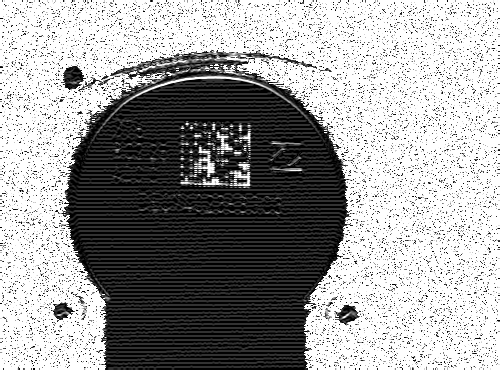
\includegraphics[width=.31\textwidth]{05_ergebnisse/ergDeflektometrischeRegistrierung/durchlichtAuswertungDeflektometrischeRegistrierung/figures/brillenglas_4_ableitung}};
		
		% Captions
		\node [below=0.2cm of img1] (cap1) {Brillenglas 1};
		\node [below=0.2cm of img2] (cap2) {Brillenglas 2};
		\node [below=0.2cm of img3] (cap3) {Brillenglas 4};			
	\end{tikzpicture}
\end{adjustbox}
\caption[Ableitung der deflektometrischen Registrierung der Zeilen bei der Durchlichtauswertung]{Ableitung der deflektometrischen Registrierung der Zeilen bei der Durchlichtauswertung.}
		\label{tikz:abbAbleitungRegistrierungDurchlicht}
	\end{figure}
}

%TODO Text
}

% Spiegelbildauswertung
{
	\FloatBarrier
    \subsection{Spiegelbildauswertung}
    \label{sub:spiegelbildAuswertungDeflektometrischeRegistrierung}
    Das Verfahren zur Bestimmung der deflektometrischen Registrierung konnte bestimmte Fehlstellen auch bei der Durchlichtauswertung sichtbar machen.
Allerdings sind schwächere Kratzer und Gravuren untergegangen.
Aus dem Grund wird zum Vergleich das Brillenglas 1 untersucht und durch den Aufbau für die Spiegelbildauswertung (siehe rechtes Teilbild aus Abbildung \ref{tikz:abbAufbauFotos}) geprüft, ob bessere Ergebnisse erzielt werden können.
Wie auch im Abschnitt \ref{sub:spiegelbildAuswertungLichtstreuung} kann für Brillenglas 1 der Rückseitenreflex durch den Polarisationsfilter und der Färbung nahezu vollständig vermieden werden.
Die Spiegelbildauswertung ermöglicht auch die Anwendung des Verfahrens für nicht-transparente spiegelnde Objekte, weshalb die Keramikobjekte 1 und 2 aus Abbildung \ref{tikz:abbStreifenaufnahmenSpLichtstreuung} zur Prüfung herangezogen werden.

\p
In Abbildung \ref{tikz:abbSinusStreifenmusterSpiegel} werden die Prüfobjekte unter der Spiegelung eines sinusoidalen Streifenmusters nach den Parametern aus Tabelle \ref{tab:paramDeflektometrischRegistrierung} dargestellt.

% Abbildung: Aufnahmen mit sinusoidalen Streifenmustern
{
	\begin{figure}[H]
		\centering
		\begin{adjustbox}{width=\textwidth}
	\begin{tikzpicture}[every node/.style={inner sep=0,outer sep=0}]
		% Bilder
		\node [anchor=north west] (img1) at (0,0) {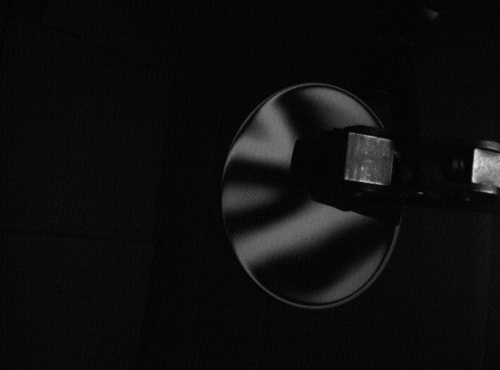
\includegraphics[width=.31\textwidth]{05_ergebnisse/ergDeflektometrischeRegistrierung/spiegelbildAuswertungDeflektometrischeRegistrierung/figures/brillenglas_1_streifenmuster}};
		
		\node [anchor=north west] (img2) at (0.345\textwidth,0) {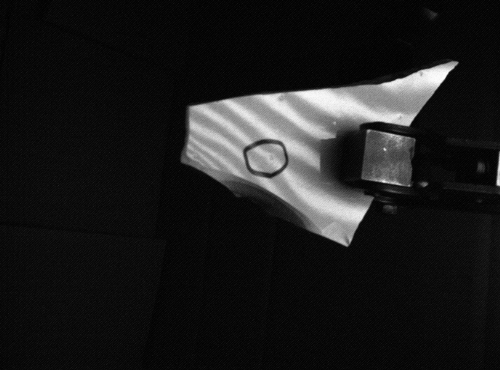
\includegraphics[width=.31\textwidth]{05_ergebnisse/ergDeflektometrischeRegistrierung/spiegelbildAuswertungDeflektometrischeRegistrierung/figures/keramikobjekt_1_streifenmuster}};
		
		\node [anchor=north west] (img3) at (0.69\textwidth,0) {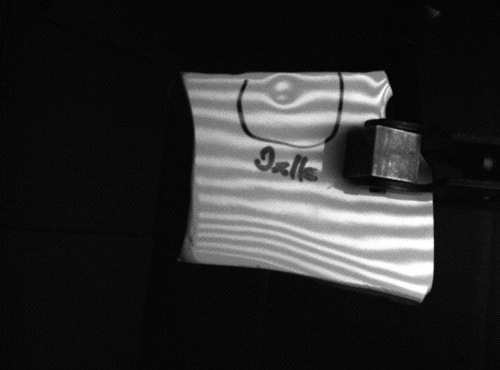
\includegraphics[width=.31\textwidth]{05_ergebnisse/ergDeflektometrischeRegistrierung/spiegelbildAuswertungDeflektometrischeRegistrierung/figures/keramikobjekt_2_streifenmuster}};
		
		% Captions
		\node [below=0.2cm of img1] (cap1) {Brillenglas 1};
		\node [below=0.2cm of img2] (cap2) {Keramikobjekt 1};
		\node [below=0.2cm of img3] (cap3) {Keramikobjekt 2};
	\end{tikzpicture}
\end{adjustbox}
\caption[Aufnahmen der Prüfobjekte unter Spiegelung der sinusoidalen Streifenmuster]{Aufnahmen der Prüfobjekte unter Spiegelung der sinusoidalen Streifenmuster}
		\label{tikz:abbSinusStreifenmusterSpiegel}
	\end{figure}
}

\noindent
Nach der Bestimmung der deflektometrischen Registrierungen der Prüfobjekte können daraus Bilder erstellt werden (siehe Definition \ref{def:graphDeflektometrischeRegistrierung}):

% Abbildung: Bilder der deflektometrische Registrierung der Zeilen
{
	\begin{figure}[H]
		\centering
		\begin{adjustbox}{width=\textwidth}
	\begin{tikzpicture}[every node/.style={inner sep=0,outer sep=0}]
		% Bilder
		\node [anchor=north west] (img1) at (0,0) {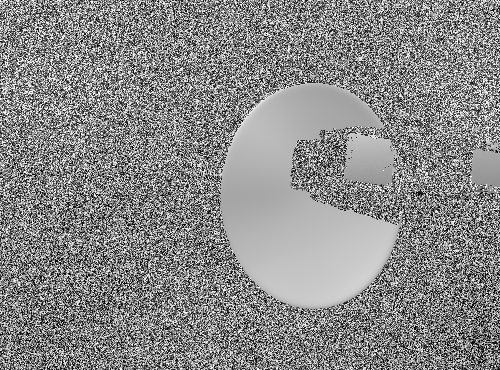
\includegraphics[width=.31\textwidth]{05_ergebnisse/ergDeflektometrischeRegistrierung/spiegelbildAuswertungDeflektometrischeRegistrierung/figures/brillenglas_1_registrierung}};
		
		\node [anchor=north west] (img2) at (0.345\textwidth,0) {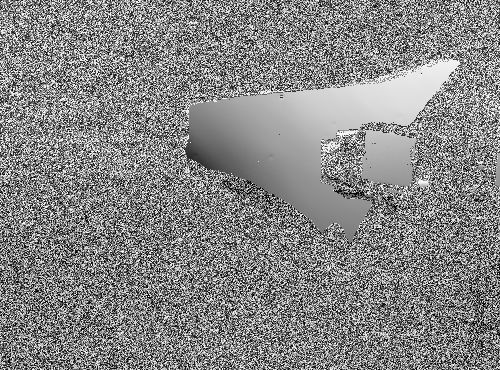
\includegraphics[width=.31\textwidth]{05_ergebnisse/ergDeflektometrischeRegistrierung/spiegelbildAuswertungDeflektometrischeRegistrierung/figures/keramikobjekt_1_registrierung}};
		
		\node [anchor=north west] (img3) at (0.69\textwidth,0) {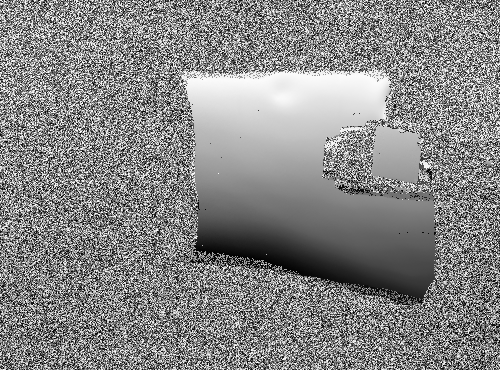
\includegraphics[width=.31\textwidth]{05_ergebnisse/ergDeflektometrischeRegistrierung/spiegelbildAuswertungDeflektometrischeRegistrierung/figures/keramikobjekt_2_registrierung}};
		
		% Captions
		\node [below=0.2cm of img1] (cap1) {Brillenglas 1};
		\node [below=0.2cm of img2] (cap2) {Keramikobjekt 1};
		\node [below=0.2cm of img3] (cap3) {Keramikobjekt 2};
	\end{tikzpicture}
\end{adjustbox}
\caption[Bilder der deflektometrischen Registrierung der Zeilen bei der Spiegelbildauswertung]{Bilder der deflektometrischen Registrierung der Zeilen bei der Spiegelbildauswertung.}
		\label{tikz:abbDeflectometricRegistrationsSpiegel}
	\end{figure}
}

\noindent
In den Bildern der deflektometrischen Zeilenregistrierung tauchen in den zu untersuchenden Objekten einzelne Bildpunkte auf, deren Grauwerte nicht zu der Umgebung passen.
Diese Ausreißer haben für die Oberflächenform keine größere Bedeutung und entstehen z. B. durch Messfehler, Fremdlicht oder die angestrahlte Abschirmung, die von innen Licht auf das Prüfobjekt reflektiert.
Durch Anwendung des Medianfilters zur Glättung des Bildes, kann man diese Störungen weitgehend entfernen.
Anschließend kann auch für diese Objekte zur Auswertung der deflektometrischen Registrierung die Ableitung der geglätteten Bilder in Richtung der Zeilen gebildet werden:

% Abbildung: Bilder der Ableitung der deflektometrische Registrierung der Zeilen
{
	\begin{figure}[H]
		\centering
		\begin{adjustbox}{width=\textwidth}
	\begin{tikzpicture}[every node/.style={inner sep=0,outer sep=0}]
		% Bilder
		\node [anchor=north west] (img1) at (0,0) {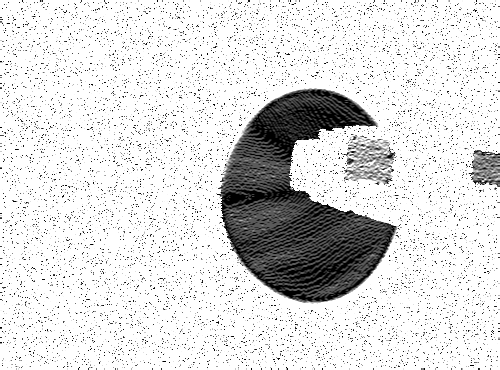
\includegraphics[width=.31\textwidth]{05_ergebnisse/ergDeflektometrischeRegistrierung/spiegelbildAuswertungDeflektometrischeRegistrierung/figures/brillenglas_1_ableitung}};
		
		\node [anchor=north west] (img2) at (0.345\textwidth,0) {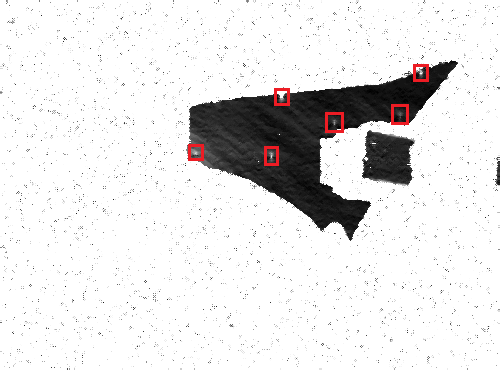
\includegraphics[width=.31\textwidth]{05_ergebnisse/ergDeflektometrischeRegistrierung/spiegelbildAuswertungDeflektometrischeRegistrierung/figures/keramikobjekt_1_ableitung}};
		
		\node [anchor=north west] (img3) at (0.69\textwidth,0) {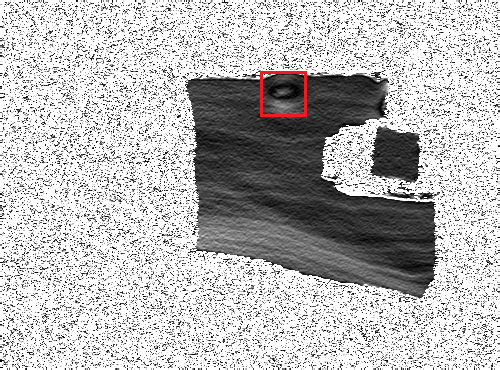
\includegraphics[width=.31\textwidth]{05_ergebnisse/ergDeflektometrischeRegistrierung/spiegelbildAuswertungDeflektometrischeRegistrierung/figures/keramikobjekt_2_ableitung}};
		
		% Captions
		\node [below=0.2cm of img1] (cap1) {Brillenglas 1};
		\node [below=0.2cm of img2] (cap2) {Keramikobjekt 1};
		\node [below=0.2cm of img3] (cap3) {Keramikobjekt 2};
	\end{tikzpicture}
\end{adjustbox}
\caption[Ableitungen der Bilder der deflektometrischen Registrierung der Zeilen bei der Spiegelbildauswertung]{Ableitung der Bilder der deflektometrischen Registrierung der Zeilen bei der Spiegelbildauswertung.}
		\label{tikz:abbAbleitungRegistrierungSpiegel}
	\end{figure}
}

\noindent
Genau wie bei der Durchlichtauswertung durch dieses Verfahren, lassen sich bei dem Brillenglas 1 in Abbildung \ref{tikz:abbAbleitungRegistrierungSpiegel} keine größeren Auffälligkeiten feststellen.
Es lassen sich demnach nicht wie im Abschnitt \ref{sub:spiegelbildAuswertungLichtstreuung} Fehlstellen oder die Gravur der Brillenkennzeichnung erkennen.
Auf den Keramikobjekten 1 und 2 erkennt man Abweichungen von den Krümmungsverläufen der Oberfläche.
In Abbildung \ref{tikz:abbAbleitungRegistrierungSpiegel} sind diese Auffälligkeiten durch rote Rechtecke markiert.
Beim Keramikobjekt 1 handelt es sich hierbei um sogenannte  \glqq Pickel\grqq ~auf der Oberfläche.
Auf der Oberfläche des Keramikobjekts 2 befindet sich im roten Rechteck eine Delle bzw. Wölbung.

\p
Als Alternative zur Auswertung der deflektometrischen Registrierung über die Ableitung, wird eine Auswertung über die Krümmungsberechnung durch den sogenannten \glqq Mexican Hat\grqq -Operator\footnote{
Der \glqq Mexican Hat\grqq -Operator bzw. der Laplace of Gaussian kann verwendet werden um die zweite Ableitung eines Bildes zu berechnen.
} durchgeführt:

% Abbildung: Bilder des Mexican Hat Filter angewandt auf die deflektometrische Registrierung der Zeilen
{
	\begin{figure}[H]
		\centering
		\begin{adjustbox}{width=\textwidth}
	\begin{tikzpicture}[every node/.style={inner sep=0,outer sep=0}]
		% Bilder
		\node [anchor=north west] (img1) at (0,0) {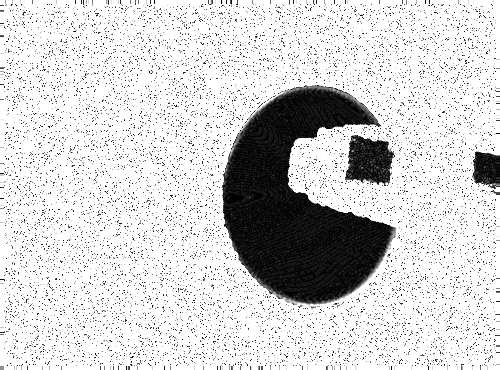
\includegraphics[width=.31\textwidth]{05_ergebnisse/ergDeflektometrischeRegistrierung/spiegelbildAuswertungDeflektometrischeRegistrierung/figures/brillenglas_1_mexican}};
		
		\node [anchor=north west] (img2) at (0.345\textwidth,0) {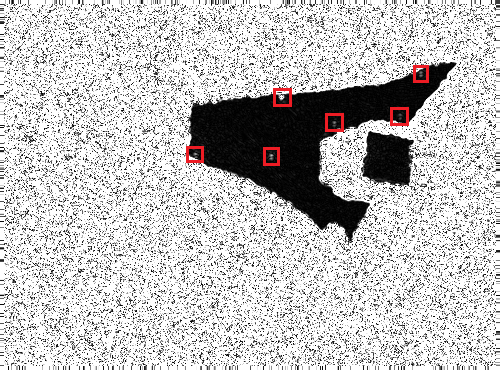
\includegraphics[width=.31\textwidth]{05_ergebnisse/ergDeflektometrischeRegistrierung/spiegelbildAuswertungDeflektometrischeRegistrierung/figures/keramikobjekt_1_mexican}};
		
		\node [anchor=north west] (img3) at (0.69\textwidth,0) {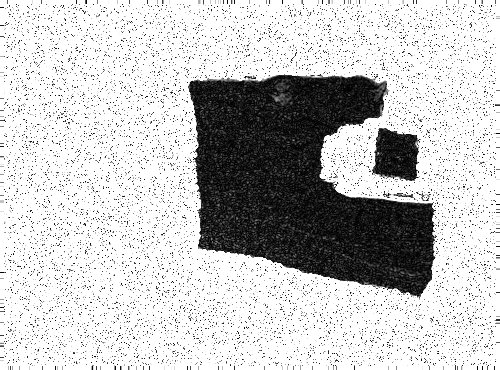
\includegraphics[width=.31\textwidth]{05_ergebnisse/ergDeflektometrischeRegistrierung/spiegelbildAuswertungDeflektometrischeRegistrierung/figures/keramikobjekt_2_mexican}};
		
		% Captions
		\node [below=0.2cm of img1] (cap1) {Brillenglas 1};
		\node [below=0.2cm of img2] (cap2) {Keramikobjekt 1};
		\node [below=0.2cm of img3] (cap3) {Keramikobjekt 2};
	\end{tikzpicture}
\end{adjustbox}
\caption[Mexican Hat-Filter angewandt auf die Bilder der deflektometrischen Registrierung der Zeilen]{Mexican Hat-Filter angewandt auf die Bilder der deflektometrischen Registrierung der Zeilen.}
		\label{tikz:abbMexicanHatRegistrierung}
	\end{figure}
}

\noindent
Auch in Abbildung \ref{tikz:abbMexicanHatRegistrierung} erkennt man im Brillenglas keine Abweichungen der Oberflächen\-krümmung.
Auf den Keramikobjekten 1 und 2 erkennt man an den in Abbildung \ref{tikz:abbAbleitungRegistrierungSpiegel} markierten Fehlstellen auch Auffälligkeiten in Abbildung \ref{tikz:abbMexicanHatRegistrierung}.
}